% Chapter 3

\chapter{Spatial microsimulation and its application to transport problems}
\label{Chapter3}
% \lhead{Chapter 3. \emph{Spatial microsimulation and % Definitely worth writing
% % as a stand-alone paper
% its application to transport problems}} % Write in your own chapter title to set
\fancyhead[RO,LE]{Chapter 3. Spatial microsimulation} %2side
\fancyhead[RE,LO]{\thepage}

\begin{quote}
\textit{The modellers' task is to predict how people and organisations will live
in
`good' and `sustainable' cities; how the infrastructure will, or should, grow;
and how activities and traffic flows are, where appropriate, best managed,
priced and regulated.}
\flushright{\citep[p.~3]{Wilson1998-past}}
\end{quote}

Microsimulation can have variable meanings depending on whether you are a
geographer, transport planner, or economist
(see \citealp{Ballas2005b, Liu2006, Bourguignon2006} for examples).
This chapter reviews existing work that uses individual level data and modelling
techniques to investigate transport and related problems.
It also introduces static spatial microsimulation, a particular type of
microsimulation that is central to the thesis. The method enables
individual level and geographical variation in commuting behaviour
to be analysed in tandem. Operational definitions, based on
established research, are important for clarity, repeatability and to
show how the work presented here builds on past research. A number of key terms will be
frequently used throughout the thesis, so this chapter begins with
definitions.
This is followed by an overview of the history (\cref{s:history}) and current
state of the art (\cref{s:sotart}) of the technique as it relates to transport
issues such as travel to work.

As implied in the quotation above, transport does not happen in isolation from
other phenomena. It is part of the complex web of social relations, the environment,
infrastructures, economics, policies and decisions
that define modern settlements. From this
perspective, spatial microsimulation for transport applications is just one
branch of a long-standing tradition of urban modelling
\citep{Wilson1970, batty1976urban, batty2007cities}.
Other branches include dedicated transport modelling techniques
(e.g.~\citealp{SATURN2012}), integrated land-use transport  models
\citep{Wegener2009} and agent-based approaches \citep{Gilbert2008-abm}.
These research areas are related to the thesis and in some cases have
the potential to build on its results. In this chapter they are
are grouped together under the broad term `urban modelling' and
discussed in \cref{s:urbanmodel}. The final section of
this chapter (\cref{s:bigdata-gps}) summarises the literature and
explains how it relates to methods implemented in the thesis.

% considers new research directions that have
% been made possible by  the availability of `big data' harvested from the
% internet or alternative sources such as GPS loans to survey participants.
% New approaches are already
% making substantial contributions to understandings of personal travel.
% Harnessed correctly, these new data sources have the potential to improve the
% energy use estimates resulting from microsimulation models and shed insight into
% the validity of assumptions made. %%%!!! Not any more!

\section{Definitions: what is spatial microsimulation?}
\label{s:defs}
\emph{Microsimulation}, as its name suggests, refers to the modelling of
individual units --- e.g.~people, household, companies --- which operate in a
wider system. Used in this sense, the term originates in economics, where it
signified a theoretical turn away from aggregate level analyses and towards a
focus on individual behaviour. ``This shift of focus, from sectors of the
economy to the individual decision making units is the basis of all
microsimulation work that has followed from Orcutt's work''
(\citealp[p.~145]{Holm1987}; see \cref{s:digirev} for further reference to
this work). Microsimulation overall therefore has a wide meaning, from
individual vehicles in a transport model \citep{Liu2006, Ferguson2012}
to the inventories of
competing firms over time \citep{Bergmann1990a}.
The term has a narrower definition in this
thesis, however, that is more concerned with modelling the distribution of
behaviours of individuals over space than over time. This thesis is predominantly
concerned with only one subset of microsimulation: spatial
microsimulation, modelling the distribution of individuals over
space. Within the category of \emph{spatial} microsimulation, different types
can be specified (\cref{types-msim}).

\emph{Spatial microsimulation} of the static kind can be formally
defined as
follows: the simulation of individual level variables within the geographic
zones under investigation \citep{ballas2003microsimulation-30-years, Ballas2007simb}.
The models that perform this operation have also
been referred to as `population synthesizers' \citep{Mohammadian2010}. This
term is useful in the context of transport applications, because small area
micro-population generation is only one stage of a wider process of
individual level transport modelling (\citealp{Pritchard2012}; \cref{f:msim-schematic}).

\begin{figure}[h]
 \centering
 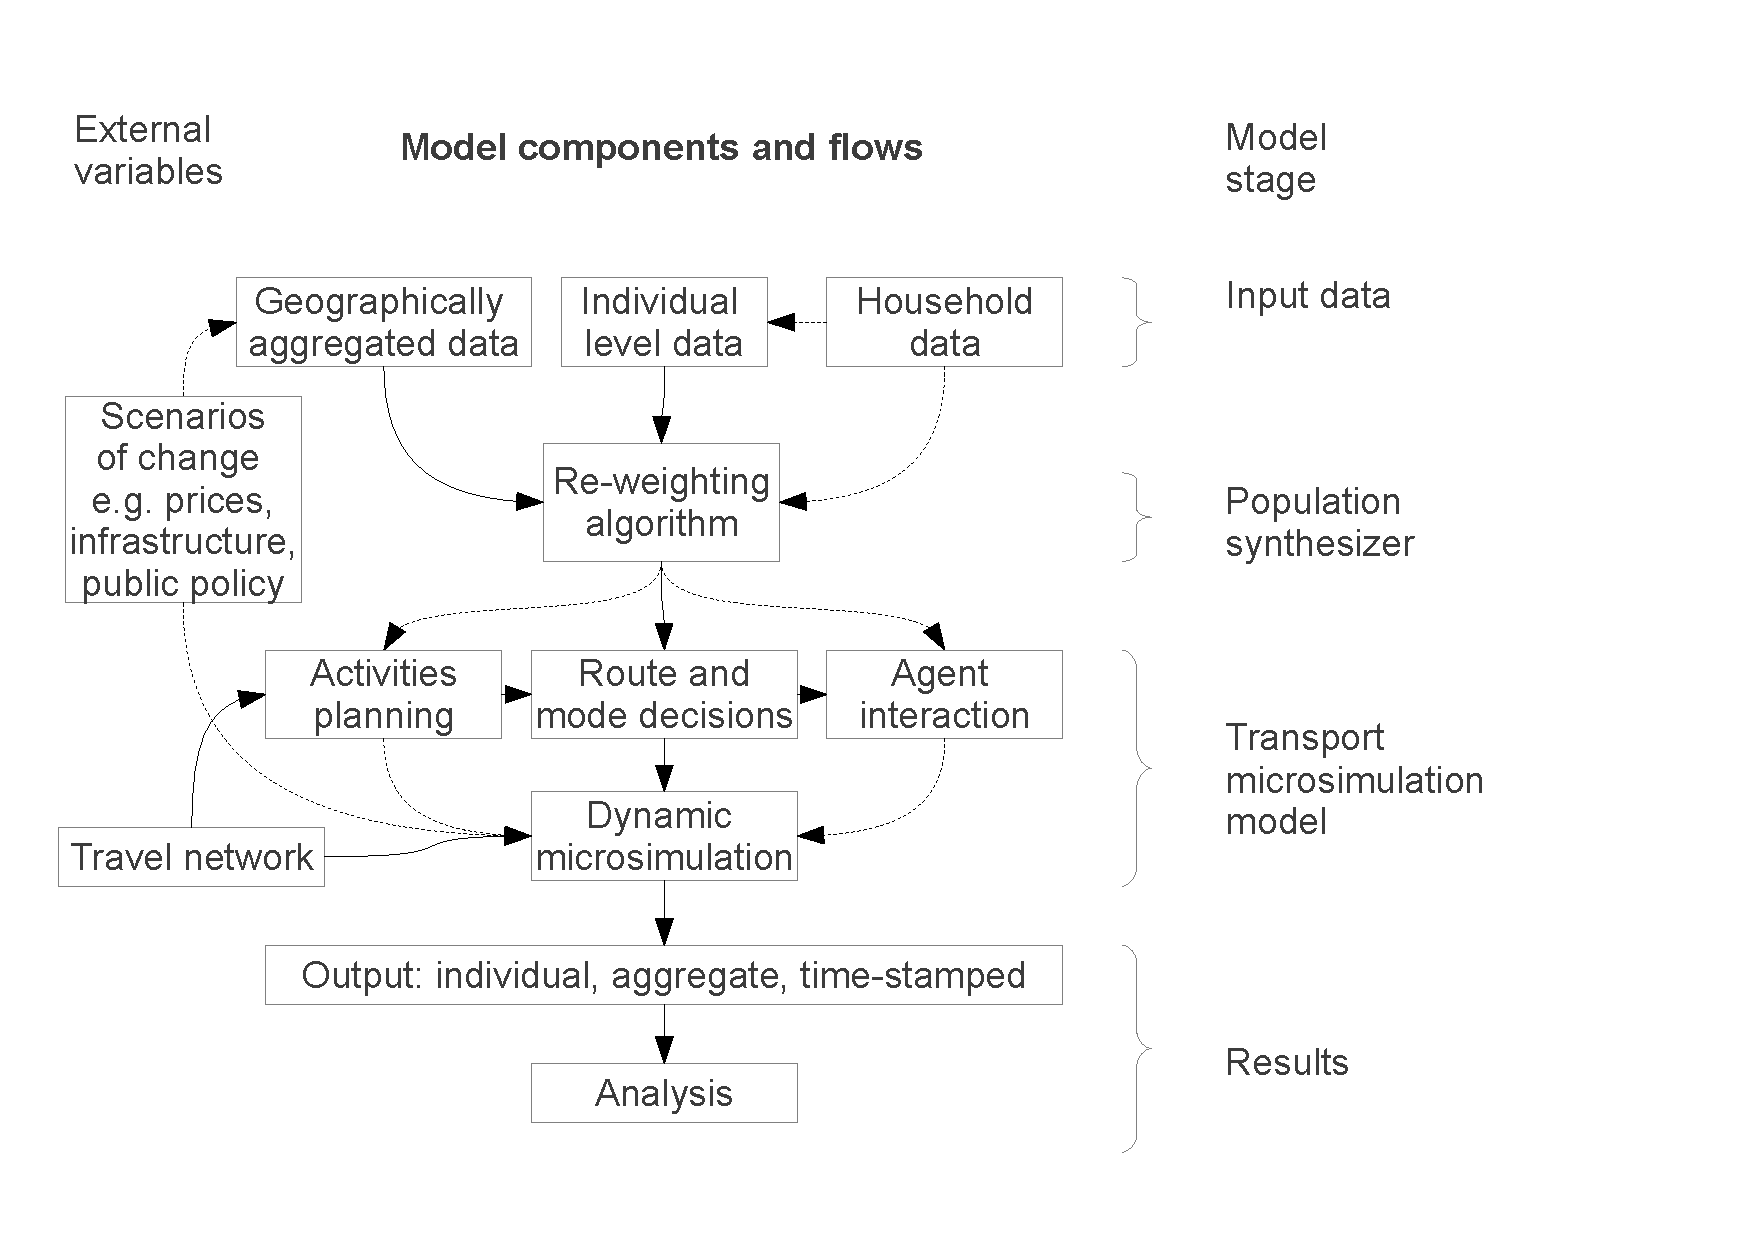
\includegraphics[width=16 cm]{msim-schematic}
 \caption[Schematic a transport simulation model]{Schematic
of the components of a complete transport simulation model such as
TRANSIMS, after \citet{nagel1999transims} and \citet{Mohammadian2010}.
This thesis is primarily concerned with the first two stages.}
 \label{f:msim-schematic}
\end{figure}

During static spatial microsimulation individuals are sampled from a non-geographical
dataset via  reweighting, based on what have become known as `constraint variables'
from early combinational optimisation work \citep{Williamson1998}. The key
feature of these variables is that they are present in
both individual level and geographically aggregated data
sets.\footnote{Constraint
variables must be categorical variables (such as
`male', `age: 16 to 19' or `works 0 to 2 km away from home')
that are shared between the micro level data and
known geographical aggregates, usually from the census.
Continuous variables have not been used in the microsimualtion
literature reviewed, although they could theoretically be
used, by constraining variables' spread, skewness
and central tendency.
}
% The next 2 paras are taken from ints3.tex
\Cref{f:msim-schematic} shows the technique in the wider context of
transport modelling. Spatial microsimulation
here refers to only the top two stages in the diagram. It represents a
computationally small but important (for social analysis at least)
part of the wider simulation process. It is important to clarify this
distinction, as the meaning of `spatial microsimulation' can be ambiguous.
It can refer
either to the process of population synthesis
\citep{chin2006regional, Ballas2005c, Hynes2008},
or the entire urban modelling process that
builds on the spatial microdata \citep{Wegener2011}.
Spatial microsimulation here refers to the former case. The results could
thus be harnessed as inputs into more complex dynamic models in which
individuals interact with each other and other entities in a wider urban model.
The terms \emph{dynamic spatial microsimulation} or \emph{agent-based models}
will be used to refer to the wider modelling process.

Static spatial microsimulation (generally and henceforth referred to simply as
spatial microsimulation) involves sampling rows of
survey data (one row per individual, household, or company) to generate lists of
individuals (or weights) for geographic zones that expand the survey to the
population of each geographic zone considered. The
problem that it overcomes is that most publicly available
census datasets are aggregated, whereas individual level data are generally
much more detailed \citep{ballas2003microsimulation-30-years}.
The ecological fallacy, whereby relationships found at one level are 
incorrectly assumed to apply to all others \citep{Openshaw1983}, for example, can be tackled
to some extent using individual level data allocated to geographical zones
\citep{Hermes2012a}. This `spatial' or `small area' microdata is the output
of spatial microsimultion.

Despite its ability to output geolocated individuals,
spatial microsimulation should never be seen as a
replacement for the `gold standard' of real,
small area microdata \citep[p.~4]{Martin2002}. From the perspective of social
scientists, it would be preferable for governments around the world to follow
Sweden's example and release such small area microdata anonymously. However, this
prospect is unlikely to materialise in the UK in the short term,
adding importance to the process
of model validation. In any case, the experience of spatial microsimulation
development and testing can help prepare researchers for the analysis of real
spatial microdata. Also, the technique's links to modelling make spatial
microsimulation useful for investigating the impacts of policy or other
changes in the real spatial microdata \citep{Holm1987}.
The method's practical usefulness (see \citealp{Tomintz2008})
and testability \citep{Edwards2009} are beyond doubt.

Assuming that the survey microdataset is representative of the
individuals living in the zones under investigation,\footnote{The suitability
of this assumption is further discussed in \cref{Chapter8}.} the
challenge can be reduced to that of optimising the fit between
the aggregated results of simulated
spatial microdata and aggregated census variables such as age
and sex \citep{Williamson1998}. These variables are often
referred to as `constraint variables' or `small area constraints'
\citep{Hermes2012a}. The term `linking variables' can also be used, as they
\emph{link} aggregate and survey data.
Based on the literature, the technique seems to have been used for five main
purposes, to:
\begin{itemize}
 \item model variables whose spatial distribution at the aggregate level is
otherwise unknown (e.g.~\citealp{Ballas1999}).
\item estimate the individual level distributions of variables within small
areas about which only aggregate counts or summary statistics are known (e.g.
distance travelled to work)
\item understand the spatial distribution of discrete behaviours
(such as visiting `stop smoking' centres --- \citealp{Tomintz2008})
and thus the likely local level effects of policy change \citep{Ballas2001}
\item project future changes at the local level, based on past trends
\citep{Ballas2005}
\item provide a foundation for agent-based models, which rely on
discrete individuals \citep{Ballas2007simb, Pritchard2012, Wu2010}
\end{itemize}
The main purposes of spatial microsimulation here are
related to bullet points one
and two above. However, elements from each will be harnessed at some
point.
In essence, spatial microsimulation merges individual level data (a list
of individuals, each with their own ID) with geographical data (a list of
zones, each with its own ID). It therefore relies on two types of input data:

The \emph{microdataset} is the individual level data from which individuals are
weighted or probabilistically selected. It is referred to as the survey
dataset \citep{Wu2008} or simply as `individual data' \citep{Simpson2005}.
The input microdata should be as representative of the zones being studied as
possible\footnote{For
example, the date of survey data collection should be
close to date of at which the zonal data was collected. Also, the survey data
should preferably be from the same geographic region as the zones under
investigation, or at least weighted so that individuals from the region under
investigation are more likely to be sampled \citep{Ballas2005-ireland}. An alternative
way of making the survey dataset more representative is to preferentially
sample individuals from areas with the same classification as the 
their zone being modelled.
}
and sufficiently diverse. %%%!!! More here!

The \emph{constraint variables}, `small area constraints' or `linking
variables' are the aggregate level variables that link the zonal and individual
datasets together. They must (for current methods, at least)
be categorical and the categories in the two
datasets must be the same (re-categorisations may be needed).

\emph{Target variables} are the variables that spatial microsimulation seeks
to estimate. Typically they are not reported at all at the small area level
(e.g.~income), leading to the term `small area estimation' being used
to describe spatial microsimulation when it is used to estimate the
average values of unreported variables for small areas. But spatial
microsimulation can also be used to simulate the distribution of variables that
are already known. Thus, although distance is a constraint variable in
our model, it is also in some ways a target variable: 
little is likely to be known about its distribution within each distance bin. 
Finally, counts of interaction
variables (e.g. male, over 50,
high social class and car driver) are typically not reported from the Census.
These can therefore also be referred to as target variables. Overall,
target variables is the term given to the information targeted for
estimation by the spatial microsimulation model.

\emph{Reweighting} is the process by which individuals are assigned a weight
for each of the zones under investigation. \citet{harland2012} provide
an overview of the methods available for this process, which is
also known as `population synthesis'. The higher the weight for a
particular area, the more representative is the individual of that area,
compared with the rest of the survey dataset. Combinational optimisation
and deterministic reweighting 
are the two main methods for reweighting \citep{Hermes2012a}.

\emph{Combinatorial optimisation} \index{combinatorial optimisation} is an
approach to reweighting that uses repeated randomised sampling to
repeatedly select individuals from the survey microdataset and allocate them to
zones \citep{Williamson1998, Voas2000}. Based on the fit between simulated
and known aggregate counts after each
iteration, the parameters of the resampling algorithm can be adjusted (e.g.~via
simulated annealing).

\emph{Deterministic reweighting} refers to non-random methods of allocating
weights to individual-zone combinations \citep{Ballas2007simb, Tomintz2008}.
Iterative proportional fitting (IPF)
is a widely used deterministic reweighting algorithm and is used in the
spatial microsimulation model throughout. Whole cases
are generated using integerisation.

\emph{Integerisation} is the process by which integer weights are generated
from the non-integer weight matrix (see \cref{s:integerisation}).

\emph{Cloned individuals} \index{cloning} are rows in the survey microdataset
that have been replicated more than once in the spatial microdataset for a
particular area \citep{Smith2009}.
The cloning of individuals can be represented by an integer
weight above one, or simply by repeating identical rows multiple times. In
practice these two forms of representing data are interchangeable; the latter
takes up more disk space \citep{Holm1996} but may make certain types of analysis
easier.


\section{The history of spatial microsimulation}
\label{s:history}
This section outlines the history of spatial microsimulation. It would
be easy to repeat past work here.\footnote{Readers interested in a
comprehensive history of the field are directed towards
\citet{Ballas2009-sage}.} To avoid this, the focus is on
developments that influence the way spatial microsimulation
is and can be used for transport applications. These include:
\begin{itemize}
 \item the influence of location on individual behaviour via
 transport costs 
 \item the question of data vs theory driven approaches
 \item converting a spatial microdataset into a behavioural model
 \item the impact of rapidly advancing computers and data sources
\end{itemize}
These themes are present throughout the section, which is ordered
roughly chronologically.

\subsection{Pre-computer origins}
The theoretical origins of spatial microsimulation stretch back to before the
turn of the 20$^{th}$ century. It was only with the emergence of large scale
data sets, methods of analysis and and conventions of mathematical notation that
quantitative analysis of variables that vary over time and space could actually
occur \citep{Ballas2009-sage}.
Despite (or perhaps partly because of) the absence of these pre-requisites for
the analysis and simulation of large populations at the individual level, much
progress was made in thinking about how individuals behave within environments
that vary in predictable ways over space before computers were available.
Consideration of travel costs (which were much higher before most
people travelled by motorised modes) was integral to both Christaller's
central place theory and Von Th\"{u}nen's concentric agricultural zones.
Lacking reliable data with which to test their ideas, the
early quantitative geographers had to make do by
developing theories based on personal observation.
Some of these theories are still influential today \citep{Clarke1985}.
Ideas developed in the pre-computer age can be seen as the theoretical
forefathers of the microsimulation models of transport behaviour, and frameworks
for interpreting the results, that are in use today.

One explanation for the greater theoretical focus of pre-computer work
is that empirical data seldom fit into any neat model and therefore
distract from explanation.
This point was made as early as the 1970s, accompanied by the
warning that the
accelerating deluge of new datasets and quantitative methods was leading some
to conflate quantification with theory \citep{Wilson1972-theoretical}.
Much theoretical work has been done since this cautionary tale. Yet the
same problems of being blinded by new information (to the detriment of
deductive thinking) face modellers now, probably to a greater extent.
This, in combination with the fame enjoyed by early theoretical geographers
(as opposed to more recent empirical geographers who modified or
rejected their work), goes a long way to explain why researchers continue to cast back to
the pre-computer age for theoretical
insight. Two of the early theories that are most pertinent to
simulation of travel patterns are Von Th\"{u}nen's, on the
spatial distribution of
agricultural activity and Christaller's central place theory.

Von Th\"{u}nen's work in the early 1800s is a seminal example of this early
theoretical thinking. His model of concentric zones of agriculture was
described verbally and in the evolving language of mathematics but rarely tested
on real data \citep{Moore1895-thesis}.\footnote{For
example, ``although [Von
Th\"{u}nen] claims that his advantage over Ricardo consists in his ability to
reduce the co-operation of capital to terms of labour, the validity of that
claim has not been tested'' \citep[p.~126]{Moore1895-thesis}.
} 
Von Th\"{u}nen's work exerts a strong
influence, even in the 21$^{st}$ century (e.g.~\citealp{lankoski2008bioenergy}) 
due to its use of geographically defined variables, strictly 
defined assumptions and extensibility \citep{sasaki2003agent}. 
The approach describes individual units based in
Cartesian space, that can be seen both as discrete zones, or as
a continuous variable (as an input into the cost of travel)
\citep{Stevens1968a}. The model's insight into the variability of
individual level behaviour depending on their zone of habitation can therefore
be seen as a direct precursor to spatial microsimulation models. These also
seek to describe the characteristics and behaviour of individual units living in
geographical zones.
%%%!!! Please god give me time to make
% A general version of the Von Thunen model and place it on github -> rinseage
% Rinse this section; concise; go back if needed!!!

Walter Christaller's central place theory of the 1930s provided an integrated
theory of spatially variable behaviour (primarily shopping) and the location of
settlements of varying sizes \citep{matthews2008geography}. Based on the
assumption of a continuous and even geographical space ready for urban growth,
the theory proved fertile for hypothesis testing and extension to other sectors.
% based on increasingly complex mathematics .
Following Von Th\"{u}nen, Christaller
attempted a `scientific' explanation of the behaviour of individuals based on
where they live. The mechanistic nature of the approach has since been
superseded by more advanced and probabilistic models
yet central place theory continues to influence
many areas of spatial modelling \citep{Wilson1972-theoretical, Sonis2005,
Farooq2012-integreted}. Applied to commuting, the theory provides a ready made
model about where people travel to work: the settlement that can provide the
best pay, minus travel costs. Of course, both pay and travel costs vary greatly
depending on a number of individual and geographic variables that cannot be known
in every case. However estimates can be made (even in the absence of now
readily available data) and applied stochastically. 
This theoretical approach has subsequently helped
explain spatial distributions in travel to work patterns, using models based on
Christaller's ideas \citep{Tabuchi2006-commuting-costs}. Christaller was
a major advocate of explaining theories in
mathematics: ``the equilibrium of the location system ... can only be
represented by a system of equations'' (Christaller, 1933; quoted in
\citealp[p.~35]{Wilson1972-theoretical}).
More recent research suggests that urban systems are rarely in equilibrium
\citep{batty2007cities}. In any case, Christaller provided a hypothesis about
why some settlements grow more than others, attracting more people, trade and
commuters.
% Whether or not this statement is true,
% and its potential applicability to commuting patterns, is
% discussed in \cref{Chapter8}. % No, it's not!
More prosaically, Christaller's theory also helps explain why
long-distance commuting appears to be more common into large cities than small ones
(see \cref{Chapter6}).
% !!! REallly? + maybe more precisely located cross ref.

The preceding discussion provides only a small snapshot of pre-computational
spatial analysis, based on two influential thinkers. The
focus was on deductive reasoning, rather than inductive methods, whereby large
amounts of data are processed in the hope of finding some underlying pattern.
This emphasis can provide a lesson for the future: despite the clear
disadvantages faced by researchers before the digital revolution, one
advantage they seem to have had was a clear theoretical focus and this may
have been due in part to absence of large and distracting datasets and
computers.
The danger that this historical perspective flags is that the masses of
micro level data now available could distract from explanation. As
\citet{Wilson1972-theoretical} emphasised, it is explanation and theory
development, not mere description, that enables a discipline to progress. 

Despite this risk, the emergence of powerful computers have allowed theories to
be developed and tested in ways that were previously impossible. The digital
revolution can thus be seen as the single most important event in the history
of spatial simulation.

\subsection{The digital revolution}
\label{s:digirev}
\begin{quote}
 At the present time, the speed and capacity
of electronic computers would still put economic limits on the number of units
that could be handled in the above fashion.
\flushright{\citep[p.~120]{Orcutt1957-new-type}}
\end{quote}

After World War II a number of factors drove interest in modelling human
behaviour and transport. Important among these were a couple of influential new
technologies: the mass produced car and electronic computers. The former
expanded rapidly in the West before the oil price shocks of the
1970s, during a sustained period of stability and economic growth. Nowhere
was this more apparent than in the USA, where the rapid uptake of the car was
forcing planners to reconsider city layouts in order to cope with the influx.
Linked to this pressure, the broadly defined art/science of `Urban Modelling'
also
began, originating in the USA \citep{batty1976urban} and continuing to this
day in a paradigm that can be described as the `science of cities' \citep{Batty2012}.

In the early phase of this research program, planning for the future
of cities in a resource-constrained world was a research priority for some,
even before the severity of environmental problems such as climate change was
fully understood \citep{Rouse1975}. The potential of numerical models to tackle
the mismatch between economic development and resource and energy issues was
not overlooked, although models were also used to investigate
how best to accommodate anticipated growth in populations, economies and
car use \citep{Irwin1973-simulation}.
Still, there were calls to harness these newly discovered methods
for consideration of the relative performance of
radically different options from first principles \citep{manheim1968search, TUI1972}.

Beyond changing mobility patterns (the impact of which was largely to provide
motivation, but not method), it was the appearance of computers that drove
forward and facilitated progress in the field. Although many now
take fast and efficient processors for granted, for example by using hand-held computers
to play `Angry Birds' and check Facebook accounts, computers increasingly are used in vital areas of
daily life, from
education to the design of traffic lights. The digital revolution should not
be seen as a single transformative event: it is an ongoing and accelerating
set of changes in the way information is stored, processed and communicated.
Combined with the internet, the digital revolution has ongoing
impacts on society \citep{Rushkoff2011}, including travel to work patterns
\citep{Orloff2003} and of course the methods available to investigate human
behaviour over space.

As with other areas of rapid technological progress, there is no
fixed point at which there is `enough' computing power to solve the
most pressing issues: an interesting phenomenon with computing power
is that, much like the problem of roads driving demand for driving up, the more
there is the more demand grows. Throughout the 20$^{th}$ century computing power
was often seen
as \emph{the} limiting factor preventing accurate simulation of social
systems.\footnote{This
is well illustrated by the quote that begins this section. To
put the quote into its proper context, consider the following: the
IBM 704 had the equivalent of 18,432 bytes of RAM. This was the first mass
produced computer and was
considered as the state of the art at the time of Orcutt's paper:
subsequently in the article it was referred to as a `powerful giant'
\citep{Orcutt1957-new-type}. Now one can purchase a laptop with 16 Gigabytes of
RAM for approximately 5\% of average UK wages (\pounds1,000). This is
1,000,000,000
times more memory than was available to the IBM, operating millions of times
faster and costing thousands of times less in real terms. Yet still people
complain about lack of computing power! In other words, as computing power has
advanced exponentially, approximately by Moore's law --- which accurately
predicts the exponential shrinkage of electronic components, by a factor of 0.7
every 3 years \citep{kish2002end} --- our hunger for more and faster processing
has increased even faster.
}
This is no longer the case: ``Modern computing is now sufficiently powerful to
deal with most [urban] models ... models based on individuals are
now feasible both in terms of their computation and their representation
using new programming languages'' \citep[p.~5]{batty2007cities}.


Regardless of our insatiable thirst for processing power, these external factors
--- the digital revolution and wider societal changes embodied in the
car --- undoubtedly drove forward research seeking to understand and model
transport systems in detail. The aim was to harness the marvel of computing
power to better understand the rapid shifts taking place.
This was most apparent in applied urban modelling: ``Increasing car
ownership during the 1940s and early 1950s led to the growing realisation
that cities with their traditional physical form could simply not cope
with the new mobility'' \citep[p.~6]{batty1976urban}. The new methods formed an
important tool for enabling planners to deal with this shift.
Some of the descendants of this early transport modelling work are described in
\cref{s:dedicated}.
%%% equations!
% after 3.2.3 drafted!

\subsection{Statistical methods for estimation}
In statistics too, more
sophisticated methods were being considered during and after World War II.
Increasingly large and complex
datasets were an additional driver of advancement here: the increased automation
and rigour of data collection led to new data management
problems. Placing his seminal work on iterative proportional fitting (IPF) in
context, \citet[p.~427]{Deming1940} provides the following example of this
data-driven methodological development:
``in the 1940 census of population a problem of adjustment arises from the fact
that although there will be a complete count of certain characters for the
individuals in the population, considerations of efficiency will limit to a
sample many of the cross-tabulations (joint distributions) of these
characters.'' In other words, IPF was developed not to simulate populations but
to fill in empty cells in situations where storing all possible cross-tabulations of
categorical data was not feasible or where internal cells needed to be
updated based on new marginal constraints:
``The iterative proportional fitting method was originally
developed not for fitting
an unsaturated model to a single body of data but for combining the information
from two or more sets of data'' \citep[p.~97]{bishop2007discrete}. To provide a
concrete example of this ``classical'' use of IPF, \citet{bishop2007discrete}
reproduce \citet{Friedlander1961-ipf} who updated cross-tabulations of
counts of women by age and marital status from the complete 1957 table by 1958
margins. More than 50 years later, IPF was still in use, to
tackle the same issue \citep{Jirousek1995}.

\index{entropy maximisation}
Parallel to these developments the concept of `entropy maximisation' emerged.
This method aims to ``produce the maximum-likelihood estimate --- the distribution [of cell
values] that is most likely to occur given no other constraints [on their
marginal totals] than those imposed'' \citep[p.~95]{johnston1985geography}.
Originally proposed and formalised mathematically in the field of statistical
mechanics \citep{jaynes1957information}, the concept was used to estimate
probability distributions that satisfy all conditions without making any
further assumptions about the data. ``Mathematically, the maximum entropy
distribution has the important property that no possibility is ignored; it
assigns positive weight to every situation that is not absolutely excluded by
the given information'' \citep[p.~623]{jaynes1957information}.
This definition is very similar to the maximum likelihood estimate attained
through iterative proportional fitting. The mathematics underlying entropy maximisation
is complex,
% (for a geographer at least!),
involving Lagrangian multipliers and
a series of interrelated equations containing exponentials
\citep{jaynes1957information}. Its relevance here is that it is a way of
estimating unknown probability distributions, based on a limited set of
constraints. In the language of spatial microsimulation, this means calculating
internal cell values based on marginal constraints. Thus entropy maximisation
can be used to estimate the maximum likelihood of individual level attributes
for areas about which only counts are available. Because of this, iterative
proportional fitting has been shown to be a specific form of
entropy maximisation \citep{Beckman1996, ye2009methodology, Rich2012}.

It was not until the
1990s
that IPF (and, often unconsciously, entropy maximisation) was discovered by
human geographers and
`put on the researcher's desk' \citep{Norman1999a} for spatial
microsimulation.\footnote{There
were a few earlier exceptions, including its application to
model the diffusion of Dutch Elm disease in the UK \citep{sarre1978diffusion}.
}
An early advocate was \citet{Wong1992}; early applications that produced
spatial microdata included \citet{Birkin1988}, who used IPF in combination with
Monte Carlo sampling to create completely synthetic microdata.
\citet{Ballas1999} used IPF to allocate individual level survey data to
areas.\citet{Mitchell2002} used IPF to create cross-tabulations
of categorical marginal totals to investigate the changing geography of health
inequalities in the UK.

Deming's methodological innovation was not especially outstanding in the context of
rapidly advancing 1940s statistics, but it is worth considering in more detail. The
IPF procedure that it was built upon (Deming, 1940) 
is now frequently used in spatial microsimulation models
 for automatically allocating individuals from a survey
dataset to the zones for which they are most representative.
New applications and refinements to Deming's method continued in the
proceeding years within statistics
\citep{stephan1942iterative,Friedlander1961-ipf}, although the term `iterative
proportional fitting' was only used to describe it after
\citet{Fienberg1970}. Since then, IPF has continued to be refined and applied to
various statistical problems involving the estimation of missing data, but
these advances are generally contained in a literature that is separate from
the body of work that is the focus of this
chapter.\footnote{As
a relevant
aside, history of IPF provides an interesting example of fragmentation in
academic research, as the statistical community continued to use Deming and
Stephen's method of estimating internal cell values based on known marginal
subtotals,
but using a totally different name: ``The methodology became known as `raking'
and found widespread application in sampling, especially at the US Census Bureau
and other national statistical offices''  \citet{Fienberg2007}. It is important
to note this divergence, as the statistical uses of IPF (or `raking') have the
potential to aid the technique's usage in spatial microsimulation.
}
The reasons for using IPF instead of combinatorial optimisation or other related
methods of discrete multivariate analysis described
in \citet{bishop2007discrete} include 
speed of computation, simplicity and
the guarantee of convergence \citep{Deming1940, Mosteller1968,
Fienberg1970, Wong1992, Pritchard2012}.
\citet{Rich2012} endorsed IPF over alternatives in the context of transport modelling.
Summarising past literature, they state that IPF can arrive at the same
(maximum likelihood) result as other maximum entropy (ME) approaches,
but faster: ``The popularity of the IPF is therefore mainly due to the
fact that it provides a solution which is equivalent to that of the ME approaches,
but attained in a much more computationally efficient way'' \citep{Rich2012}.

It was only with the intervention of Guy Orcutt that such methodological
advancements were combined with new computing capabilities to provide new
possibilities for social science, based on the simulation of individuals.
Although Orcutt is often cited as one of the founders of social simulation,
arguably his most important contribution was to place computerised methods in a
wider conceptual framework of policy analysis. Instead of using a
single `representative agent' with averaged values, the microsimulation method
enabled the evolution of multiple micro units to be traced, under different
scenarios \citep[p.~176]{mitton2000microsimulation}.
This helps explain why Orcutt (\citeyear{Orcutt1957-new-type,
orcutt1961microanalysis}) is frequently cited as one of the founding fathers of
the field
(e.g.~\citealp{Clarke+Longley1989-UK-housing-sim,Wu2008,
Ballas2013-4policy-analysis}). Granted, he successfully exported the concept of
manipulating individual level variables based on estimated
probabilities of change, but Orcutt was not particularly interested in
spatial analysis.\footnote{Although
Orcutt was instrumental in advocating and demonstrating
micro level methods for policy evaluation, he was more concerned with time than
he was with
space. %%%!!!referred
Neither IPF nor combinational optimisation, two of the main tools used for
generating spatial microdata in spatial microsimulation research today,
%!!!verify
are mentioned in his seminal works
\citep{Orcutt1957-new-type,orcutt1961microanalysis}.
Instead, he laid down the tantalizing possibilities of simulating society, in
very general (and seldom validated) terms, using the newly available
mainframe computers. The following is a typical example of the clarity,
enthusiasm and sense of purpose of his vision: ``The following method is
feasible, readily comprehensible and may serve to illustrate still further the
proposed model. Using this approach the model would be simulated on a large
electronic machine, such as the IBM 704 or the UNIVAC II, or some improved
successor to these powerful giants'' \citep[p.~119]{Orcutt1957-new-type}.
}
Building on Orcutt's methods, simulation grew popular in the
increasingly quantitative social sciences. Uptake was
greatest in economics, where the technique
gained a strong following as a method for evaluating the impact of
changing policy and economic conditions at the individual level
(see \citealp{Merz1994} for an overview).
The branch of microsimulation associated with spatial problems emerged later
\citep{Tanton2013-intro}, although it has clear links with earlier shifts
towards modelling within the wider field of quantitative geography
(e.g.~\citealp{Clarke1985}).

The shift to the practical application of microsimulation to explicitly
\emph{spatial} problems was not to happen until around 30 years after the
1960s applications. This can partly be attributed to the
computational limits emphasised by Guy Orcutt at the outset of this chapter, but
partly also to a disinterest in quantitative models on the part of geographers.
A seminal paper \citep{Holm1987} reviewed the limited experience of
microsimulation models for
spatial applications up to that point. The authors warned of ``the
possibility of the method being reinvented by different
researchers independently'' if the new techniques continued to be ignored by
geographers \citep[p.~145]{Holm1987} and provided a coherent argument in favour
spatial microsimulation, culminating in the following conclusion:
``With micro-modelling it is possible to use and formulate theoretical concepts
and hypotheses about social action on at least the same level of detail as
sometimes found in other social sciences  without neglecting the apparent and
important elements of spatial interdependence seldom found in studies outside
geography'' \citep[p.~163]{Holm1987}.
Thus the gauntlet was laid down to future
researchers entering this emerging field: develop spatial microsimulation models
to take advantage of newly available computers, programming languages and
datasets. Since then ``the speed of development has gathered
pace''\citep[p.~259]{clarke2013conclusions}. Spatial microsimulation is now a
field of social and spatial analysis in its own right, with an expanding range
of applications. 

\subsection{Modern spatial microsimulation}
Geographers are not generally taught computer programming.
This, and the `erosion of quantitative literacy' \citep{ESRC2013}
helps explain why spatial microsimulation has been limited to a
small field within geography and related disciplines. Spatial
microsimulation now constitutes ``a relatively small
community'' that can be considered a field in its own right
(Wilson, in \citealp[p.~vi]{Tanton2013}).

This community can roughly be identified as those with links
to the International Microsimulation Association (IMA), 
who publish spatial microsimulation work in peer reviewed
journals\footnote{The following journals are common places for the
publication of spatial microsimulation research:
\emph{Computers, Environment and Urban Systems},
\emph{The international Journal of Microsimulation},
\emph{Journal of Artificial Societies and Social Simulation} and
\emph{Environment and Planning A}. Applied spatial microsimulation
research is also published in a wide range of regional science
and geography journals.
}
and whose work is referred to in recent overviews of the field
\citep{Tanton2013, O'Donoghue2013}.
In summary, spatial microsimulation has emerged
from pre-computer origins and mid 20$^{th}$ century theoretical quantitative
geography to tackle the research challenge set out by
\citet{Holm1987}. Since powerful computers became available at the turn
of the 21$^{st}$ century, methods and applications have
proliferated and accelerated. Spatial microsimulation now
provides small-area estimates
of individual level variables and projections of future change.
Transport, along with a number of other phenomena, has been
identified as an area for future application of the modelling framework
\citep{clarke2013conclusions}.
% yet there is much scope for
% Microsimulation models clearly had great potential yet many of the researchers who
% could benefit most from them lacked the skills to `get stuck in' and build
% spatial microsimulation models from scratch. Even if scripts were made available, it
% would have been difficult to find suitable computers and programming expertise to
% run them until the turn of the century, by which time approaches to spatial microsimulation
% were moving on. Spatial microsimulation is undoubtedly a fast moving field, in which
% a number of key papers have had a large effect on subsequent studies. To gain an understanding
% of the reasons behind the current state of the art \cref{s:sotart}, seminal papers that
% have helped to consolidate and define the field are presented below:
% \begin{itemize}
%  \item \citet{Holm1987}
%  \item \citet{Williamson1998}
%  \item \citet{}
% \end{itemize}
% 
% \citep{Birkin1989}
% \citep{ballas2003microsimulation-30-years}
% % Tell a story: it started in Africa, uptake by geographers
% \citep{Wong1992}
% \citep{Johnston1993}
% 
% The first national dynamic spatial microsimulation model was the System for
% Visualising Economic and Regional Influences in Governing the
% Environment (SVERIGE) \citep{vencatasawmy1999building}. This model, unlike the
% static approach used in this PhD, is fully dynamic and includes modules which
% calculate fertility, mortality, employment and other life events including
% migration. SVERIGE focuses on agent life events, rather than the geographical
% distribution of their individual level attributes and how they were allocated to
% different
% places.\footnote{In fact, SVERIGE did not need to allocate any individuals from
% an a-spatial dataset to zones based on linking variables. This is because a
% micro level dataset containing all Swedish individuals is available to
% researchers \citep{Ballas2005-ireland}. This removes the need for
% spatial microsimulation via reweighting as defined above. 
% 
% } The dynamic nature of 
% SVERIGE and its basis in real microdata make it a powerful tool for evaluating
% the impacts of national policy changes \citep{ Ballas2013-4policy-analysis}
% 
% an early spatial agent-based model (see
% \cref{s:agent-based}), rather than as an early example of dynamic spatial
% microsimulation as described by .

\section{Spatial microsimulation: state of the art}
\label{s:sotart}
Spatial microsimulation can now be seen as a field in its own right, with roots
in Economics, Geography, Statistics and Regional Science.  It is
evolving, so any rigid definition of the `state of the art' is likely to become
obsolete quickly. Instead, the scope of spatial
microsimulation is explained below in terms of the types and applications of models
in use, the variety of reweighting algorithms and recent transport applications.

\subsection{Types of spatial microsimulation models} %%% Add applications 
\label{types-msim}
%%% Taken directly from ints paper
The wide range of methods available for spatial microsimulation can be divided
into static, dynamic, deterministic and probabilistic approaches (Table
\ref{typology}). Static approaches generate small
area microdata for one point in time. These can be classified as
either probabilistic methods which use a random number generator and
deterministic reweighting methods, which do not. The latter produce
fractional weights. Dynamic approaches project small
area microdata into the future. They typically involve modelling of
life events such as births, deaths and migration on the basis of random
sampling from known probabilities on such events \citep{Ballas2005c,
Vidyattama2010}; more advanced agent-based techniques, such as spatial
interaction models and household level phenomena, can be added to this basic
framework \citep{Wu2008, Wu2010}. There
are also `implicitly dynamic' models, which employ a static
approach to reweight an existing microdata set to match
projected change in aggregate level variables
(e.g.~\citealp{Ballas2005-ireland}).

\begin{table}[h]
\centerline{}
\caption{Typology of spatial microsimulation methods}
\vspace{0.25 cm}
\footnotesize{
\begin{tabular}{p{1.6cm}p{2.4cm}p{3.5cm}p{3.0cm}p{2cm}}
\toprule
{Type} & {Reweighting technique} & {Pros} & {Cons} &
{Example} \\ \midrule
\multirow{3}{2cm}{\vspace{0.3cm} \\ Determ-  inistic\\\vspace{0.3cm}
Re-\\weighting} & Iterative proportional fitting (IPF) & Simple, fast, accurate,
avoids local optima and random numbers & Non-integer weights &
\citep{Tomintz2008}⁠⁠ \\ \cmidrule{2- 5}
& Integerised IPF & Builds on IPF, provides integer
weights & Integerisation reduces model fit & \citep{Ballas2005c}⁠ \\
\cmidrule{2- 5}
&  GREGWT, generalised reweighting
& Fast, accurate,
avoids local optima and random numbers & Non-integer weights  &
\citep{Miranti2010}⁠ \\ \midrule
\multirow{2}{2cm}{ \\ Probab- ilistic  Combin-
atorial optim-
isation} & Hill climbing approach & The simplest solution to a combinatorial
optimisation, integer results & Can get stuck in local optima, slow &
\citep{Williamson1998}⁠ \\ \cmidrule{2-5}
& Simulated annealing & Avoids local minima, widely
used, multi level constraints & Computationally intensive
& \citep{kavroudakis2012}⁠  \\ \midrule
\multirow{2}{2cm}{\vspace{0.3cm} \\ Dynamic} & Monte Carlo
randomisation to simulate ageing  & Realistic treatement of stochastic
life events such as death & Depends on accurate estimates of life event
probabilities & \citep{Vidyattama2010}⁠ \\
\cmidrule{2- 5}
& Implicitly dynamic & Simplicity, low
computational demands & Crude, must project constraint
variables & \citep{Ballas2005b}⁠ \\ \bottomrule
\end{tabular}
}
\label{typology}
\end{table}

In practice, the typology presented in \cref{typology} is an
oversimplification. The spatial microdata generated during the same spatial
microsimulation project can be used for both static and dynamic applications and
different reweighting algorithms can be applied to the same dataset with
similar results. Spatial microsimulation can thus be seen as an evolving
process rather than a `once-through' analysis. A typical spatial microsimulation
project, for example, may involve some or all of the following four steps
(the first four are from \citealp{ballas2003microsimulation-30-years}):
\begin{itemize}
 \item construct a micro-dataset, usually from surveys
 \item reweight the individual level data to create a spatial microdataset
 \item static what-if scenarios (implicitly dynamic scenarios in
\cref{typology}) to assess the impact of instantaneous change
 \item agent-based modelling, to better understand how the individuals in each
zone interact with the environment and each other
\end{itemize}

% The applications of spatial microsimulation can also be usefully categorised
% to inform discussion on the method's expanding range of uses.
% 
% \citet{van2012multifunctional} harnessed a spatial microsimulation model
% to provide input data for a logit model of shopping preferences.
% This modelling exercise provided estimates of the
% impact of new a supermarkets on surrounding stores: it was calculated
% how much more or less would be spent in each. This novel use of
% spatial microsimulation for scenario-testing is highly policy-relevant
% (and politicised), and could be made more so by calculating distributional
% impacts.

\subsection{Reweighting algorithms} %%% Could easily put the IPF paper here
\label{sreweight}
To run a spatial microsimulation model, a prerequisite is a mechanism by
which individuals from the survey are selected to `populate' the areas under
investigation. For the technique to be worthwhile, it is vital that individuals
who are in some way representative of each area should be selected
\citep{Ballas2005}⁠. Doing this manually is clearly not feasible, so a number
of computerised techniques have been developed to create weight matrices
automatically. This section provides an overview of the reweighting techniques
that have been used in published research; the findings fit directly into the
choice of microsimulation model used in this research. %(Illustration here???)

Reweighting algorithms allocate individuals counts or weights for target
areas based on a number of matching or linking variables that are shared between
area and survey datasets. A number of options are available and these can be
broken down into the following categories:
deterministic/randomised, integer/ratio and count/weight.
The option used in this thesis is deterministic
sampling based on IPF. This reweighting procedure was
chosen due to the repeatability of the
results,\footnote{``One
advantage of a deterministic model is that the estimated population
distributions will be the same each time the model is run'' \citep{Smith2009}⁠.
Thus, the results of any model to be replicated
without the need to ``set the seed'' of a known list of
Pseodo-random numbers \citep{Robert2009}: this makes results easier to
test and update when new data emerges.}
relative simplicity and past experience with
the technique.

Randomised (combinatorial optimisation) sampling strategies have the advantage
of robustness against local
optima, which may mean that deterministic models may not always arrive at the
optimal solution \citep{Williamson1998}.
Also, a combinatorial optimisation sampling strategy has the inherent advantage of
keeping individuals as integers (as opposed to deterministic reweighting,
which results in fractional weights). This makes it easier to
understand the simulated population, analyse the results 
(e.g.~ the Gini Index calculation
is more straightforward if integer weights are used) and select
subsets of the simulated population with certain characteristics.
In addition, integer weights are needed for agent-based models. On the other
hand, integer results can be associated with large differences between simulated
and actual cell values \citep{Ballas2005}⁠.

In order to calculate the probabilities of survey individuals appearing in
statistical areas, iterative proportional fitting (IPF) has been used. By
altering the cell values in a 2 dimensional matrix, IPF is used to match
``disaggregated data from one source with the aggregated data from another''
\citep[p.~1]{Norman1999a}⁠. This is done iteratively: each iteration brings the column and
row totals of the simulated dataset closer to those of area in question.

Another, more fundamental, disadvantage of IPF is its inability to simulate
individuals based on data at multiple levels, for example household and
individual: ``it can control either for agent level or for group level
attributes but not for both simultaneously'' \citep[p.~5]{Muller2010}.
This problem has long challenged researchers because ``working at the
household/family and person levels simultaneously can introduce conflicts
between the competing goals of achieving good fit at both levels''
\citet[p.~694]{Pritchard2012}. \citet{Pritchard2012} have tackled this problem
by matching either individuals to known family attributes, for example 
based on conditional probabilities of the spouse sharing given
attributes (age, level of education). These results offer the promise of allowing
family level microdata generation from deterministic reweighting algorithms
such as IPF.

Despite the wide range of reweighting options available and even wider
range of implementations, there has been relatively little work comparing
different approaches. Most model experiments evaluate goodness-of-fit for
only a subset of reweighting algorithms, changing just one or two variables
at a time \citep{Voas2000, Smith2009, Rahman2010}. Another problem is the
wide range of evaluation tools on offer, leading to confusion about
which method is appropriate for a given application:
``Different researchers use different methods to test the
reliability of their results. This makes it more difficult for `outsiders'
to evaluate the value of a model or set of artificial population data''
\citep[p.282]{Hermes2012a}. This issue is tackled with respect
to the problem of integerisation in \cref{s:integerisation}
and discussed in more general terms in \cref{meval}. One group
of `outsiders' that could benefit from more accessible code and
reproducible testing of it is the transport community, who are increasingly
turning to spatial microsimulation to meet the need to include
social factors in scenario evaluation.

\subsection{Transport applications}
%%% This is the section I need to write next 4 this chap. First I'd like some results.
It was mentioned in \cref{s:defs} that `population synthesis' is a synonym for
(static) spatial microsimulation. The term is used by transport modellers
to describe the
process of generating individuals as inputs into wider transport models.
Thus spatial microsimulation is used in transport applications.
Whether to classify any given transport study as spatial microsimulation for
transport analysis, or a transport model with spatial microsimulation
`bolted on', is a question of semantics not dwelt on
here.\footnote{\citet{Ballas2013-4policy-analysis}
treat activity-based
transport models as an add-on to spatial microsimulation methods.
The approach taken here is to deal with 
spatial microsimulation models that have some transport
considerations added-on (this section) separately from
dedicated transport models  that also simulate individuals
(\cref{s:dedicated}).}
In any case, there is clearly a
large degree of overlap between
the two approaches. This section describes transport research that focuses on the
individual (human, not vehicle) level, primarily through spatial microsimulation.
\Cref{s:dedicated} outlines dedicated transport models, which can also harness
spatial microsimulation data as an addition to assess social impacts.

Transport modelling has a long history with strong links to engineering
,\footnote{The strength of engineers'
influence is emphasised in the following passage: ``If the main brief
of the planners is to recommend the `shape' of cities,
then it is usually left to the engineers to design, build and manage the
transport systems. Engineers,
therefore, can use models as design tools: for predicting loads ...
network optimisation ... they will have concerns with project
appraisal'' \citep[p.~16]{Wilson1998-past}.}
strategic planing \citep{Wilson1998-past} and hence large contracts.
Aggregate economic return on income has thus played a central role in
project evaluation and has become a focus of various modelling efforts
\citep{Masser1992}.
Perhaps due to this narrow technical and economic heritage, traffic models
have tended to omit people from the analysis. Technical
questions, such as `how much congestion will intervention x alleviate?',
predominate, rather
than social questions more common in spatial microsimulation research
such as `which groups will benefit most from intervention x?'.
Thus it has been rare for socio-economic variables to be included in
the model-based evaluation of transport projects, although
social impacts are increasingly considered \citep{Masser1992, Tribby2012}.
This explains growing interest
in spatial microsimulation for transport applications.
It is in this context --- a divide between the transport community, with its focus
on traffic and aggregate economic performance and the spatial microsimulation
community, with its focus on distributional impacts and public policy --- that these
studies are conducted. 


\citet{Pritchard2012} advocated harnessing spatial microsimulation
for methodological reasons, including the computational benefits of sparse data storage
for transport models.\footnote{Sparse storage here refers to data structures
whereby only non-zero values are stored and replication
weights are used instead of repeating statistically identical individuals multiple
times. This also avoids problems associated with arbitrary categories, e.g.~for
age: ``Complete array storage is proportional to the number of categories used
for each attributes, while the sparse storage scheme is not affected by the
categorization of the attributes'' \citep[p.~691]{Pritchard2012}.} These
efficient % could add table 1 from here - cool!!!
data structures have origins in early spatial microsimulation
research \citep{Holm1987, Williamson1998} and have the additional benefit
of providing ready-made inputs into agent-based transport models such as
ILUTE (see \cref{s:dedicated}).


\emph{PopGen} is a program used
to generate spatial micro-data on the characteristics of individuals
living, and using transport services, in the study region
\citep{Ravulaparthy2011}. It \index{PopGen}
is essentially a static spatial microsimulation model that combines non-spatial
survey data with `marginal tables'
(constraint variables). Three input files can be used at each level ---
individual, household and optional `groupquarters'
(these are generally students living away from home) --- leading to a high level of
detail. The use of iterative proportional updating (IPU) is key to the
ability of PopGen to simultaneously match individual and household level
characteristics, during the process of allocating individuals to household
\citep{ye2009methodology}. PopGen is made freely available to
anyone from Arizona State University and has been used as a population
synthesizer for other tranpsort studies \citep{pendyala2012application}.

\emph{Popgen-T} is a different (albeit confusingly similar in name) population
synthesiser developed specifically for the purpose of analysing the
distributional impacts of new transport schemes such as congestion charges
\citep{Bonsall2005}. The method uses IPF to combine data from a very wide range
of sources, although the exact mechanism is not
explained.\footnote{In the 2005 paper, the following information on
data sources was provided: ``The data sources used in this application include the
Household Census, the National Travel Survey, the Journey to Work Census,
the Household Income Survey, The Household Expenditure Survey,
the New Earnings Survey and a number of local travel surveys'' \citep[p.~410]{Bonsall2005}.
The data are further explained in a 2002 working paper, but this could not
be found.} Since the 2005 paper, no further implementations of the Popgen-T method
could be found.




\section{Microsimulation in urban modelling}
\label{s:urbanmodel}
Urban modelling goes beyond the estimation of individual level
characteristics, as performed in spatial microsimulation.
It attempts to include influential factors from the entirety of
urban experience, from house prices and the labour market to
the transport network and land-use. It is therefore inherently
an ambitious project, that could claim to encapsulate transport models
and explain travel to work patterns in their wider context.
Only recently have data and computational power emerged to
make this `dream' reality; many of the approaches to urban
modelling are related to this research. The most relevant are outlined below.

Five entities central to any urban model have been identified
% by Wilson (2000),
by \citet{wilson2000complex} and
it is the interaction between these that determines
the final model outcome. The importance of each
for influencing commuter flows, level of data availability and
ease of incorporation into quantitative models is presented in
\cref{t:entities}. Ultimately, these considerations should determine
whether, and at what stage, each of these entities are included in urban models.
\begin{table}[htbp]
\caption{Five entities central to urban modelling, after Wilson (2000)}
\begin{tabular}{p{2cm}p{3.5cm}p{3.5cm}p{3.5cm}} \toprule
Entity & Data availability & Importance for commuter flows & Ease of model inclusion \\ \midrule
People & High: commuting data collected in the Census and surveys & High: personal behaviour & High: individuals are basic unit of analysis \\
Organisations & Low: rapid change (especially in private sector operators) and poor accountability in many cases & Medium: councils and companies influence travel patterns & Low: organisations often
diffuse bodies \\
Commodities, goods, services & Low: petrol sales and bus ticket data not publicly available & Medium: travel is effected by price of fuel & Medium: can be defined by price of oil; depends on
elasticity \\
Land & High: maps of terrain and land use readily available & Medium: network distance and terrain alter travel behaviour & Medium: via influence of topology and distance \\
Infrastructure & Medium: Open Street Map and Ordnance Survey data & High: personal travel depends on infrastructure & Medium: can influence local travel decisions \\
\bottomrule
\end{tabular}
\label{t:entities}
\end{table}
Based on the basic multi-criteria analysis presented in
\cref{t:entities}, the following
hierarchy of entities for inclusion was established, in descending order
order of priority:

$people > infrastructure > land > commodities > organisations$.

This priority list was considered when 
compiling the data in \cref{Chapter4},
although only the first and second are
included in the methods of this thesis. Due to the importance of road network
planning, much of the research in the broader field of urban modelling is
dedicated to the development of dedicated transport models, which focus on
the second element of Wilson's (2000) list.
% The available data are therefore presented in this order, after a
% brief discussion of an additional data source that is
% vital to the research problem: energy use in transport.

% \subsection{Agent based models} %!!! Add this at some point
\label{s:agent-based}
\subsection{Dedicated transport models}
\label{s:dedicated}
Transport modelling is a large field within the wider framework of
urban modelling. It has a long history, but has undergone a rapid
evolution in the last decade, largely due to the emergence of the
internet, which allows large collaborative software projects to flourish.
Three dedicated transport models, of increasing levels of sophistication
have been selected from the
vast array of options to illustrate the state of transport modelling
and its relation to this thesis
(see \citealp{Rasouli2012} for a technical review).

\emph{SATURN} is a commercial transport model, originally
developed at the University of
Leeds \citep{boxill2000evaluation}. Its current incarnation
is version 11, a stable package running only on Windows \citep{SATURN2012}.
The SATURN model is a mature tool for determining traffic loads on road
networks given a known origin-destination flow matrix,
and is used for this purpose in local authorities in the UK
\citep{boyce2005urban}.

\emph{OpenTraffic} addresses many of the issues arising from commercial,
closed-source traffic simulation models such as SATURN: ``Most commercial
traffic simulation packages primarily offer only ready-to-use
functionality and do not facilitate the addition of new
functionality by users or provide a transparent picture of how the
underlying components are implemented'' \citep[44]{Tamminga2012}.
This recently developed simulation framework has a modular design
and is therefore useful in a wide range of applications, from
`car follow' to activity planning \citep{Tamminga2012}.

\emph{MATSim} is a more mature open source transport model that improves
on previous transport modelling programmes in a number of ways
\citep{rieser2007agent}. \index{MATSim}
The model allows individual attributes to be maintained throughout
agent-based simulation and ensures that trips made throughout the
day are realistically inter-dependent (see \cref{fmatsim-schema} for the
model's structure). For example, being late for one trip
will have an impact on the start-time of the next \citep{Balmer2009}.
Since the project was first made available as a free open source project
in 2006 (see \href{http://sourceforge.net/projects/matsim/files/MATSim/}{sourceforge.net}),
uptake has been rapid with applications ranging from agent-based
modelling of trips for leisure and shopping \citep{horni2009location}
to intensive
performance testing, in which MATSim is shown to accurately
model real world travel patterns \citep{balmer2008agenta, gao2010comparison}.
MATSim has also been used to model commuter patterns in Pretoria, South Africa,
incorporating previously omitted trip-chaining behaviours \citep{van2011agent}.

\begin{figure}[hb] \centerline{
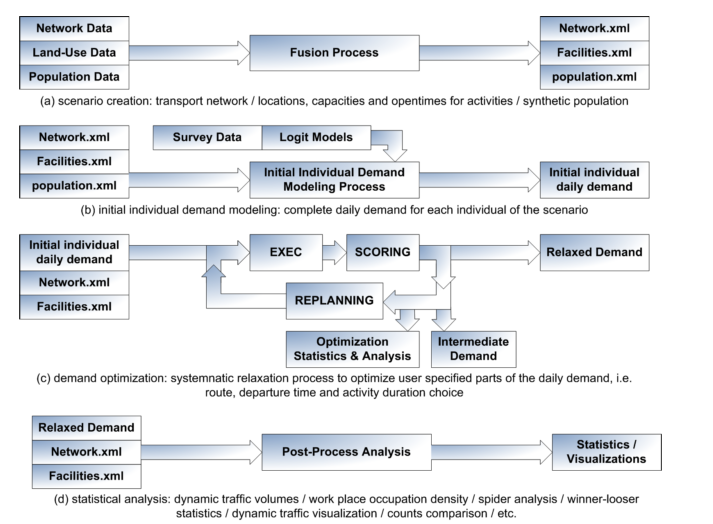
\includegraphics[width=14cm]{matsim-schema}}
\caption[MATSim schema (permission: Michael Balmer)]{Schema of the MATSim
model \citep{Balmer2009}. Thanks to Michael Balmer for permission.}
\label{fmatsim-schema}
\end{figure}

Because MATSim builds on Kai Nagel's experience as a computer scientist, who
also developed the highly successful TRANSIMS model (described below),
it has several advantages over competitors. These include:
\begin{itemize}
 \item ``MATSim is consistently constructed around the notion that travellers
 (and possibly other objects of the simulation, such as traffic lights) are `agents',
 which means that all information for the agent should always kept together in
 the simulation at one place'' \citep[p.~9]{Balmer2009}. This allows demographic
 data on each traveller to be instantly available, rather than being completely
 unavailable (as in most transport models),
 or available in a fractured file system (as in TRANSIMS).
 \item MATSim is fast to run in comparison with other transport
 models with similar specifications.
 \item Strong user community. As of May 2013, there is a comprehensive
 new tutorial on how to install and use MATSim (see
 \href{http://www.matsim.org/docs/tutorials/}{MATSim.org's tutorials site}),
 and daily commits to the source
 code (see \href{http://sourceforge.net/apps/trac/matsim/timeline}{sourceforge.net}).
\end{itemize}
For these reasons, and due to its accessibility to anyone with a modern computer,
MATSim has been identified as the most appropriate pre-existing model for
interacting with the data and methods presented in this thesis. MATSim
was carefully designed from the ground up to be the most powerful, user-friendly
and fast agent-based transport model available. It is important to recognise
that in order to avoid trying to `re-invent the
wheel'.\footnote{See \cref{s:workdes}
for a crude attempt to integrate the road network in the spatial microsimulation
--- a MATSim implementation may have been more appropriate given sufficient
time.
}
% Insert here an image of MATSim (Balmer2009) and where my model fits in 

\subsection{Land-use transport models}
% ``The first generation urban models were designed and implemented in
% North America mainly during the years 1959-68, years which coincided
% with the launching of large-scale land-use-transportation studies in major
% metropolitan areas.''
Researchers now have decades of experience modelling individual agents
\citep{Ortuzar1982},
transport flows \citep{Wilson1970} and the land-uses that lead personal
transit to take place \citep{batty1976urban}.
Of course, each of these elements depends to some extent on the others, so
integrated land-use transport models have long been regarded as the holy grail
in urban modelling. It is only recently that the computational
requirements of this task have been
available.\footnote{The memory requirements alone of storing a detailed
transport network in RAM are large. Combining this with complex polygons
defining administrative zones, a detailed microdataset and then performing
calculations defining how each model object changes from one moment to the next
in high temporal resolution is clearly a taxing computational task.
}
Despite the daunting complexity and data and computational requirements of such
models, their design and implementation has been theorised and attempted
since the 1960s, with limited levels of success
\citep{timmermans2003saga}. The author of this critical review went so far as
to suggest that the costs invested in ambitious land-use transport models
generally outweigh the benefits.
% ``There seems insufficient support for
% such investment, especially because the field has not succeeded
% in commercialising the short-term forecasts of traffic flows''
% \citep[p.~3]{timmermans2003saga}.
On the other hand, some have argued that it is only with modern computers and software
that integrated land-use transport models can move from a mere
`dream' \citep{timmermans2003saga}  into reality: ``recently,
the development of large-scale integrated land-use and
transportation microsimulation systems such as ILUTE ... ILUMASS
... and UrbanSim has generated a new excitement in the field'' \citep[p.~935]{Pinjari2011}.
These models, and TRANSIMS, are outlined below.

% A number of integrated models have been developed
% \emph{RAMBLAS}

\emph{ILUTE} \index{ILUTE} represents the `third wave' of transport-land use
models based on individual level data:
``[it] represents an experiment in the development of a
fully microsimulation modelling
framework for the comprehensive, integrated modelling of urban transportation-land use
interactions and, among other outputs, the environmental impacts of these interactions''
\citep[p.~15]{timmermans2003saga}. Thus ILUTE can can be used to analyse a wide range
of phenomena: it is an integrated urban model in the fullest sense of the word
and has been even been used to analyse the distribution of house prices
in and large city over time \citep{Farooq2012-integreted}.

%\emph{TRESIS}
\emph{UrbanSim}, like ILUTE, is a micro level integrated land-use transport
model, aimed at \index{UrbanSim}
``incorporating the interactions between land use, transportation, the economy,
and the environment'' (\href{http://www.urbansim.org/Main/WebHome}{urbansim.org}, 2012).
The source code (written in Java and Python)
is open source and remains under continued development \citep{Nicolai2012-matsim}.
Perhaps because the software is free for anyone to download, use and modify,
it has been used for a range of applications including as a tool
to aid planners in the evaluation of transport projects \citep{Borning2008}.
Although UrbanSim does not contain an advanced transport module,
work has been done to integrate the dedicated transport MATSim model (see
\cref{s:dedicated}) into it,
via a plug-in \citep{Nicolai2012-matsim}.

\emph{TRANSIMS} \index{TRANSIMS} was developed at the Los Alamos National
Laboratory with an
ambitious objective mirroring that of ILUTE:
``to model all aspects of human behaviour related to
transport in one consistent simulation framework''
\citep[p.~1]{nagel1999transims}.  The model, which is based on cellular
automata, has been given a public licence (the NASA Open Source Agreement
Version 1.3), is cross-platform (with Windows and Linux binaries) and has been
widely adopted.\footnote{``TRANSIMS''
was cited 166 time in Google
Scholar in 2012 publications, many of which implemented the model for their own
applications.}
% It would be good to have ``n. times cited, 2012'' as a variable in comp. tab.
The encouragement of community contributions and an experienced development team
has led the model to be extended various ways. For example, TRANSIMS can be
configured to take advantage of parallel processing (in which one CPU is
allocated to each area being modelled) \citep{nagel2001parallel}, or external
programs for the visualisation of results
(http://sourceforge.net/projects/transimsstudio). The sub-modules of TRANSIMS
include a micro level population synthesizer, a trip generator, route planner
and microsimulator (which determines the location and behaviour of each
individual at each time step). The model is being increasingly adopted by
Municipal Planning Organizations (MPOs) in the USA \citep{lawe2009transims,
ullah2011travel} and has successfully simulated the entirety of Swiss travel
flows (around 10 million trips), using a `Beowulf cluster' of parallel computers
\citep{Raney2003}.

The modular design of TRANSIMS means it can be used in conjunction with the
spatial microsimulation methods presented in this paper. The small area
microdata could, when allocated home-work pairs, be used as an input forming
the baseline situation at time zero. The potential for combining the spatial
microsimulation methods presented in this thesis with additional modelling
tools is described in chapter 8.
% !!! Include this !!!

\section{Summary: research directions and applications}
\label{s:bigdata-gps}
Over time the uses of spatial microsimulation, in its broadest sense,
have expanded from a way of
providing quantitative geographers and others with individual level data, into a more
general modelling strategy harnessed to tackle many problems.
In this thesis, however, a narrower definition is used:
spatial microsimulation here refers to the process of generating spatial
microdata, analogous to `population synthesis' in transport models.
As in many fields, the
rate of change has also increased, due to increased availability of
sophisticated software, large datasets and powerful
computers. One could make the argument that the
uses of spatial microsimulation, as defined above, have become more specialised
as it is adopted by various fields for their own purposes, sometimes under
different names. This fragmentation is aggravated by the fact that
many do not make the code used for their analysis available, a
practice prevalent across the sciences \citep{Ince2012}.
However, there are also signs of integration. With the continued growth of
open source software and the greater dissemination of code
(e.g.~through sites such as Github), a kind of evolutionary process can be observed:
winners are picked and then generalised to be applied to a range of
problems.\footnote{A
good example of this positive-feedback process of picking winners, whereby
the most promising projects receive much new attention and then grow most
rapidly as a result (of peer feedback and new collaborators), is MATSim.
Released as an open source project in 2006, the project has rapidly gained
users, contributors and policy applications. MATSim also illustrates the
wide appeal of microsimulation software, finding applications as ranging from
a `plugin' to pre-existing urban simulation models to a framework for
modelling leisure and shopping trips \citep{Nicolai2012-matsim, horni2009location}.
}
% \citep{Clarke2013-concs}

The rate of change is fast, yet it is important to make use of more than 30 years
. Looking back, it is possible to reflect
on what works and what does not work so well in spatial microsimulation
research. Summarising a large body of experience,
\citet[p.~197]{Holm2013-design-principles} created the following `wish list' of
factors that future spatial microsimulation researchers should consider
when creating new, or updating existing, models:
\begin{itemize}
\item  use the most modern software
\item  use standard methods, shared by many users
\item  backward compatibility (so keeping our old models and subsystems running)
\item  avoid relearning
\item  develop solutions that are theoretically well designed
\item  transfer knowledge and know-how to new colleagues
\end{itemize}
It is interesting to note that this list could have been as applicable 30 years
ago as it is now, indicating key areas of continuity in the field.
Effort has been invested throughout to comply with these
principles. It is hoped that the focus on the final point, dissemination of methods,
will enable spatial microsimulation to be used by policy
makers.\footnote{To
this end, experiments to improve the performance of IPF and some other
script files that may be of use to others
have been put online via the dissemination portals www.rpubs.com/robinlovelace
and www.github.com/robinlovelace . Knowledge transfer was also behind the
publication of a user manual alongside \citet{Lovelace2013-trs}.
}
Indeed,
its potential for policy evaluation, at individual and local levels, was
one of the major reasons for choosing the spatial microsimulation approach
to tackle the problem, helping to fill the `scale gap' between academic
studies and policy interventions described in \cref{Chapter2}.

The literature summarised in this chapter should make it clear that
the methods used are not new: researchers have been modelling
transport problems at the individual level over two decades \citep{Ortuzar1982},
and developing the theory behind individual level behaviour for even longer
\citep{Wilson1970}.
The novel
contribution made in this thesis is the practical \emph{application} of
the existing method of spatial microsimulation to the problem of unsustainable
commuting. Approaching the issue from a quantitative geography and spatial
microsimulation perspective allows the focus on spatial
variability and social inequalities in transport energy use, highlighted in
\cref{Chapter6} to \cref{Chapter8} of this thesis. This is in contrast to the 
transport modelling perspective, which is still largely traffic-orientated.
Before proceeding to apply
the method, however, it is vital to understand precisely how the
spatial microsimulation model used in this thesis works and the input data.
That is the task of the next chapter.



%!!! include these!!!
% \subsection{`Big data'}
% \subsection{GPS-loan surveys}
% \subsection{Applications for model validation and enhancement}
\label{s:applications}

%%%%%%%%%%%%%%%%%%%%%%%%%%%%%% Deshets
% In economics, spatial microsimulation has been used to \citep{Cullinan2011}
